\chapter{Lösungsansatz}
Das folgende Kapitel beschreibt den nötigen Lösungsansatz der späteren Konzeptentwicklung.

\section{Fachkonzept}

\subsubsection{Anforderungen}
Die zu entwickelnde Anwendung soll ein Anwendungszenario für die neu erschlossenen Anwendungsgebiete des \ac{poc}s umsetzen.
Die Anwendung muss dabei eine Vielzahl an Anforderungen erfüllen.
Die Software muss einfach Ausliefern und bereitzustellen sein.
Dieser Prozess muss vor inbetriebnahme automatischen verlaufen und eine individuelle Konfiguration anbieten.
Weiterhin muss bestimmtbar sein auf welchen Ressourcentyp die Anwendung bereitgestellt wird.
Die Anwendung muss Skalierbar sein und mit der Infrastruktur wachsen können.
Sie muss auch die Verwaltung von Datensätzen ermöglichen.
Auch die Kommunikation zwischen anderen Anwendung muss möglich sein.
Die Software muss auch Testprozesse unterlaufen, um die Funktionalität sicherzustellen.


\subsubsection{Blaupause}
Ein weiterer Schwerpunkt ist die Blaupausenartige Umsetzung der Software Architektur für die moderne Infrastruktur.
Die Entwicklung der Anwendung muss so gestaltet werden, dass zukünftige Projekte auf diese aufbauen können.
Ansätze bei der Entwicklung müssen austauschbar sein und in Teilschritte zerlegt werden.


\section{Grobkonzeption}
In diesem Abschnitt wird die grundlegende Idee anhand des Fachkonzepts formuliert.
Danach folgen die groben Teilschritte zur Realisierung der Testanwendung.


\subsection{Grundlegende Idee}\label{idee}

Die prototypische Anwendung wird containerisiert und über eine Container-Registry verfügbar sein. 
Weiterhin muss die Anwendung unter der Berücksichtigung der Aspekte einer Microservice-Architektur, wie in Abschnitt \ref{Microservice} beschrieben, konzipiert und entwickelt werden. 
Die einzelnen Dienste der Anwendung müssen auf einem Kubernetes-fähigen Cluster ausgeliefert und in Betrieb genommen werden.
Bevor die Anwendung verwendet wird, muss ein fester Testprozess die Funktionalität gewährleisten.

Für die mögliche Auslieferung bei einem Kunden der Krones AG soll die Nutzung bereits vorhandener Hardware mit Grafikkarten möglich sein. 
Es ist vorgesehen, dass die Anwendung in einem hybriden Cloud-Szenario die vordefinierte Hardware nutzen kann. Folglich soll die Verwendung der Hardware zu einer verbesserten Leistungsauswertung von Modellen im Bereich der künstlichen Intelligenz führen. 
Arbeitslasten, wie dem Auswerten von Deep-Learning-Modellen wie im Falle der Linatronic AI \cite{linatronic}, sollen beispielhaft dargestellt werden. 
Dafür muss die Kommunikation von Diensten in Echtzeit stattfinden, um Informationen am Zielort schnell zu verarbeiten und eine nahtlose Verarbeitung großer Daten zu ermöglichen.

\subsubsection{Anwendungsszenario}\label{Anwendungsszenario}

Der Schwerpunkt der zu entwickelnden Anwendung soll ein Dashboard mit Authentifizierungsmechanismus sein. 
Dieser soll Benutzern ermöglichen sich mit ihrem Passwort in ihr Profil einzuloggen. 
Dabei besteht auch die Möglichkeit eine Zwei-Faktor-Authentifizierung zu aktivieren und sich per Gesichtserkennung einzuloggen.
Die Daten sollen persistent gespeichert werden und können bei erneutem Aufruf der Website wieder verwendet werden. 

\subsubsection{Blaupause}

Die Anwendung soll nachvollziehbar entwickelt werden und als Fundament für spätere Entwicklungen dienen.
Softwarekomponenten der Anwendung müssen austauschbar sein und mit unterschiedlichen Technologien ersetzt werden können.
Schnittstellen müssen für gängige Kommunikationsprotokolle entwickelt werden.

\newpage

\subsection{Infrastruktur}
Auf der Grundlage von Abschnitt \ref{idee} werden die Grobentwürfe erstellt.
Die Konzeptentwürfe gliedern sich in zwei Teile, der Infrastruktur und der Anwendung.

Die Abbildung \ref{fig:GrobentwurfInfrastruktur} stellt das Zielsystem dar.
\begin{figure}[!htb]
  \centering
  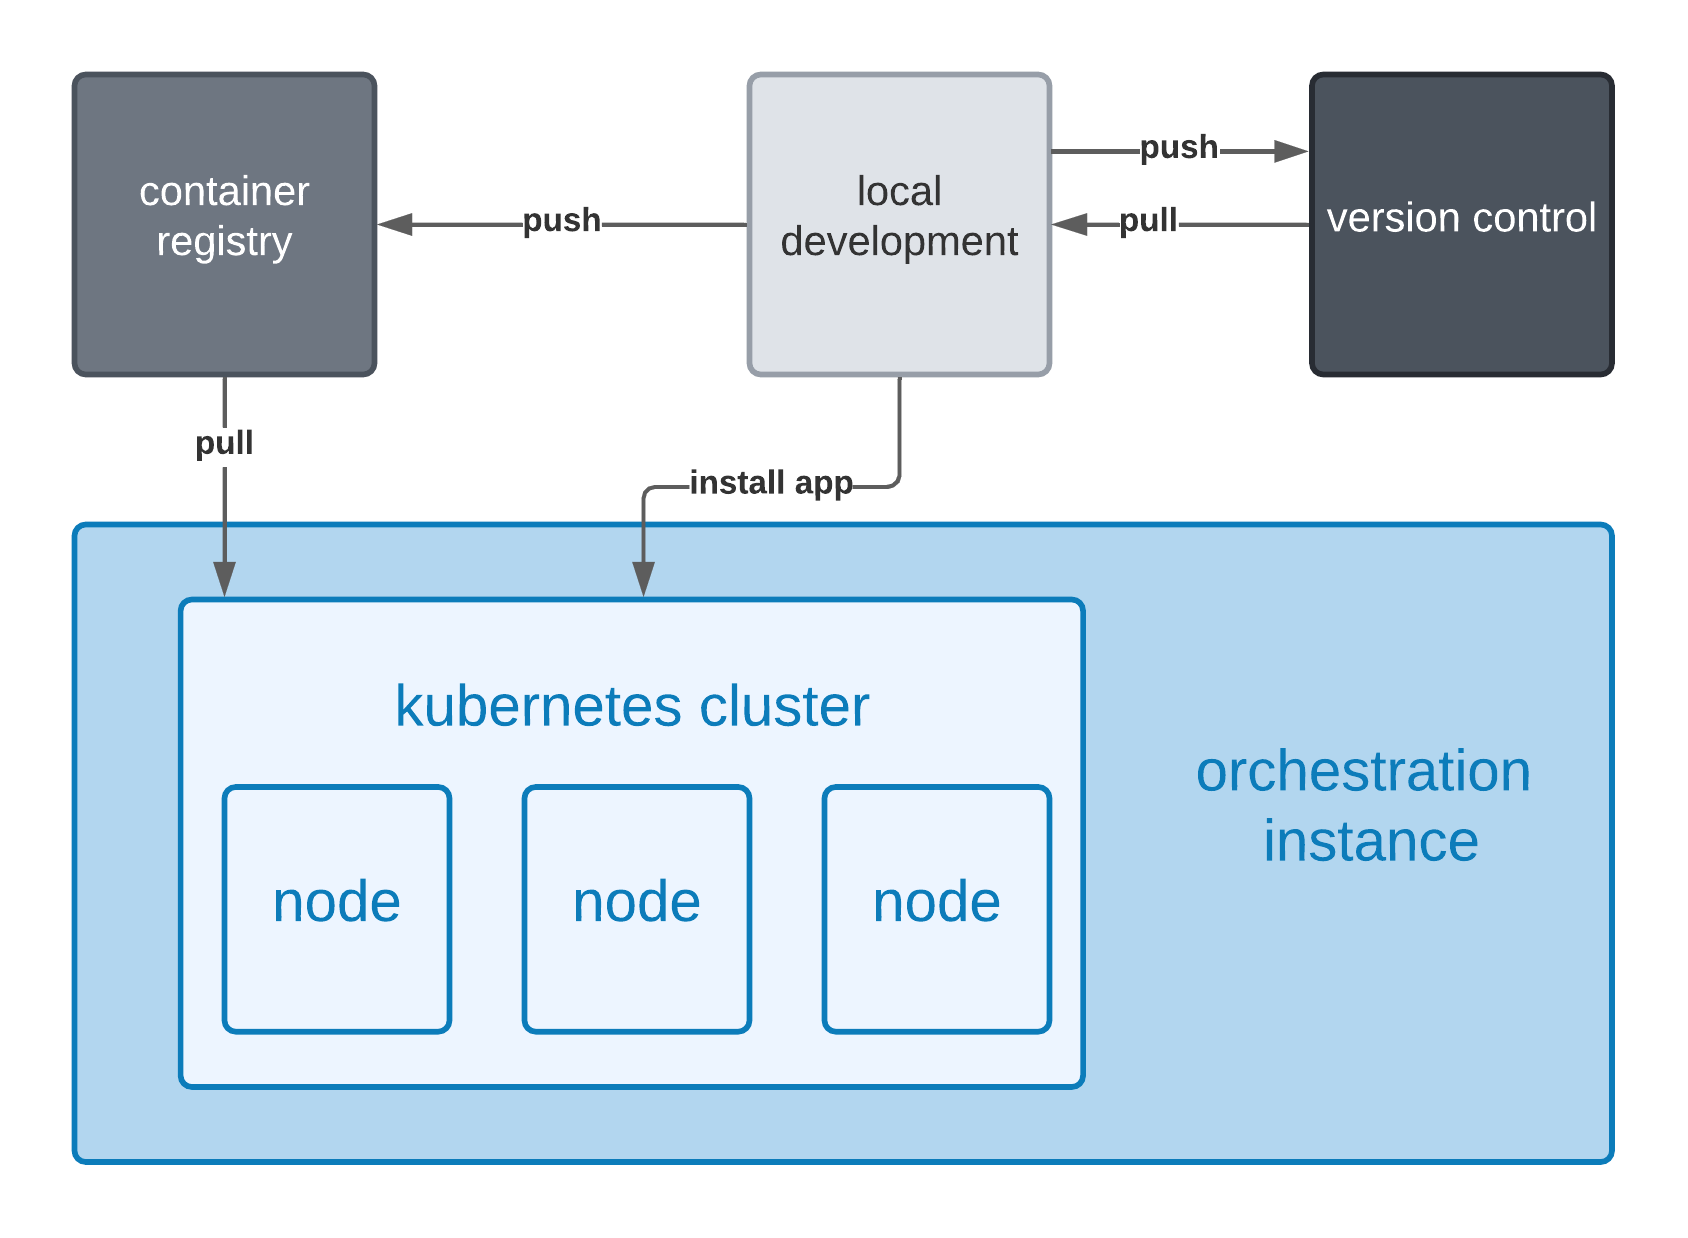
\includegraphics[width=0.8\columnwidth]{images/GrobentwurfInfrastruktur.png}
  \caption{Grobentwurf der Infrastruktur}
  \label{fig:GrobentwurfInfrastruktur}
\end{figure}

\textbf{Lokale Entwicklungsumgebung}: Die Entwicklung der Anwendung verläuft lokal und wird durch ein Versionsverwaltungssystem verwaltet.
Ein Befehl an das Kubernetes-Cluster initialisiert die Auslieferung und Bereitstellung der einzelnen Dienste. 

\textbf{Image-Registry}: Für die Auslieferung und Bereitstellung von Containern wird ein Image-Registry verwendet.
Dienste erhalten seperate Images und können unabhängig abgerufen werden.

\textbf{Kubernetes-Cluster}: Das Kubernetes-Cluster wird von einer Orchestierungsinstanz verwaltet.
Das Abrufen der Dienste erfolgt über ein Image-Registry.





\subsection{Anwendung}
Die Abbildung \ref{fig:GrobentwurfAnwendung} stellt das Anwendungszenario aus dem Unterabschnitt \ref{Anwendungsszenario} dar.
Die Anwendung aus dem Szenario wird in drei Dienste aufgeteilt.

\begin{figure}[!htb]
  \centering
  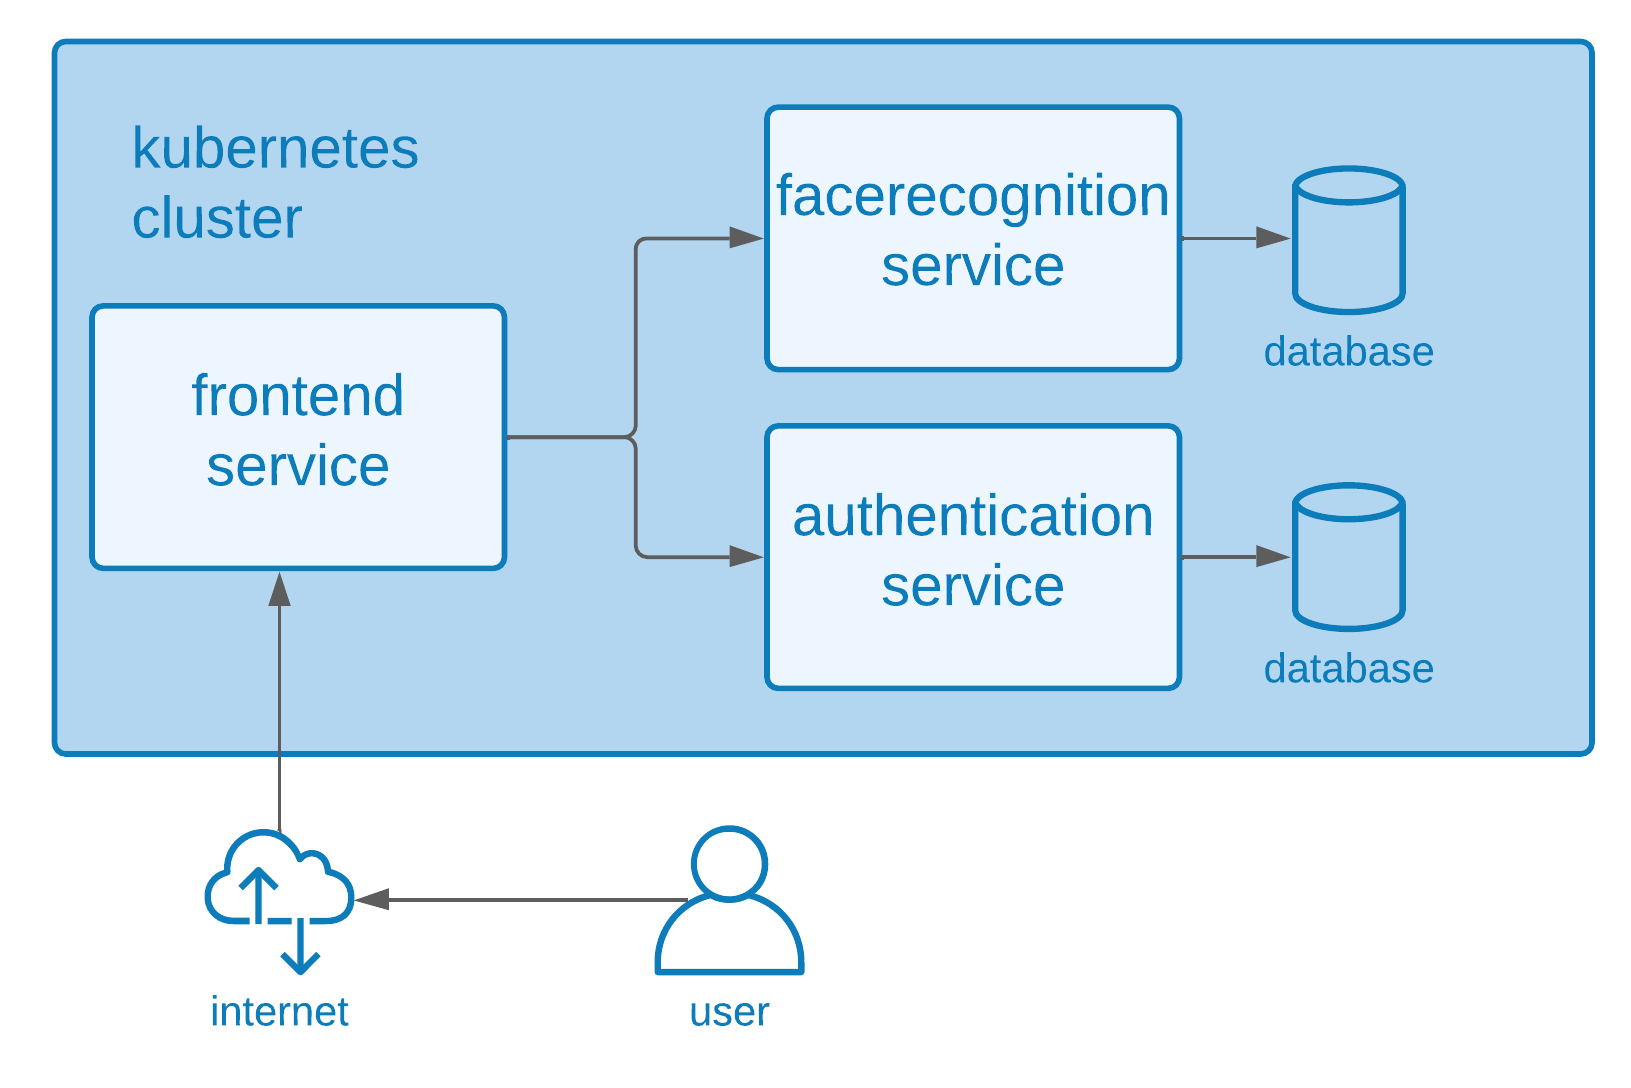
\includegraphics[width=0.8\columnwidth]{images/GrobentwurfAnwendung.png}
  \caption{Grobentwurf der Awendung}
  \label{fig:GrobentwurfAnwendung}
\end{figure}

\textbf{Frontend-Service}: Das Dashboard wird über den Frontend-Service bereitgestellt.
Darüber kann ein Benutzer die Funktionalitäten anderer Dienste nutzen.

\textbf{Authentication-Service}: Die Anmeldung und Registrierung in ein Nutzerkonto erfolgt über den Authentication-Service.
Dieser ermöglicht die persistente Speicherung der Nutzerdaten.

\textbf{Facedetection-Service}: Der Facedetection-Service bietet eine Anmeldung mithilfe von Gesichtserkennung an.
Die relevanten Daten zur Gesichtserkennung werden in einer Datenbank persistent gespeichert.

\subsection{Entwicklungsprozess}

Die Entwicklung der Anwendung wird in vier auf sich aufbauende Schichten eingeteilt (vgl. Abbildung~\ref{fig:Schichtenentwurf}).

\begin{figure}[!htb]
    \centering
    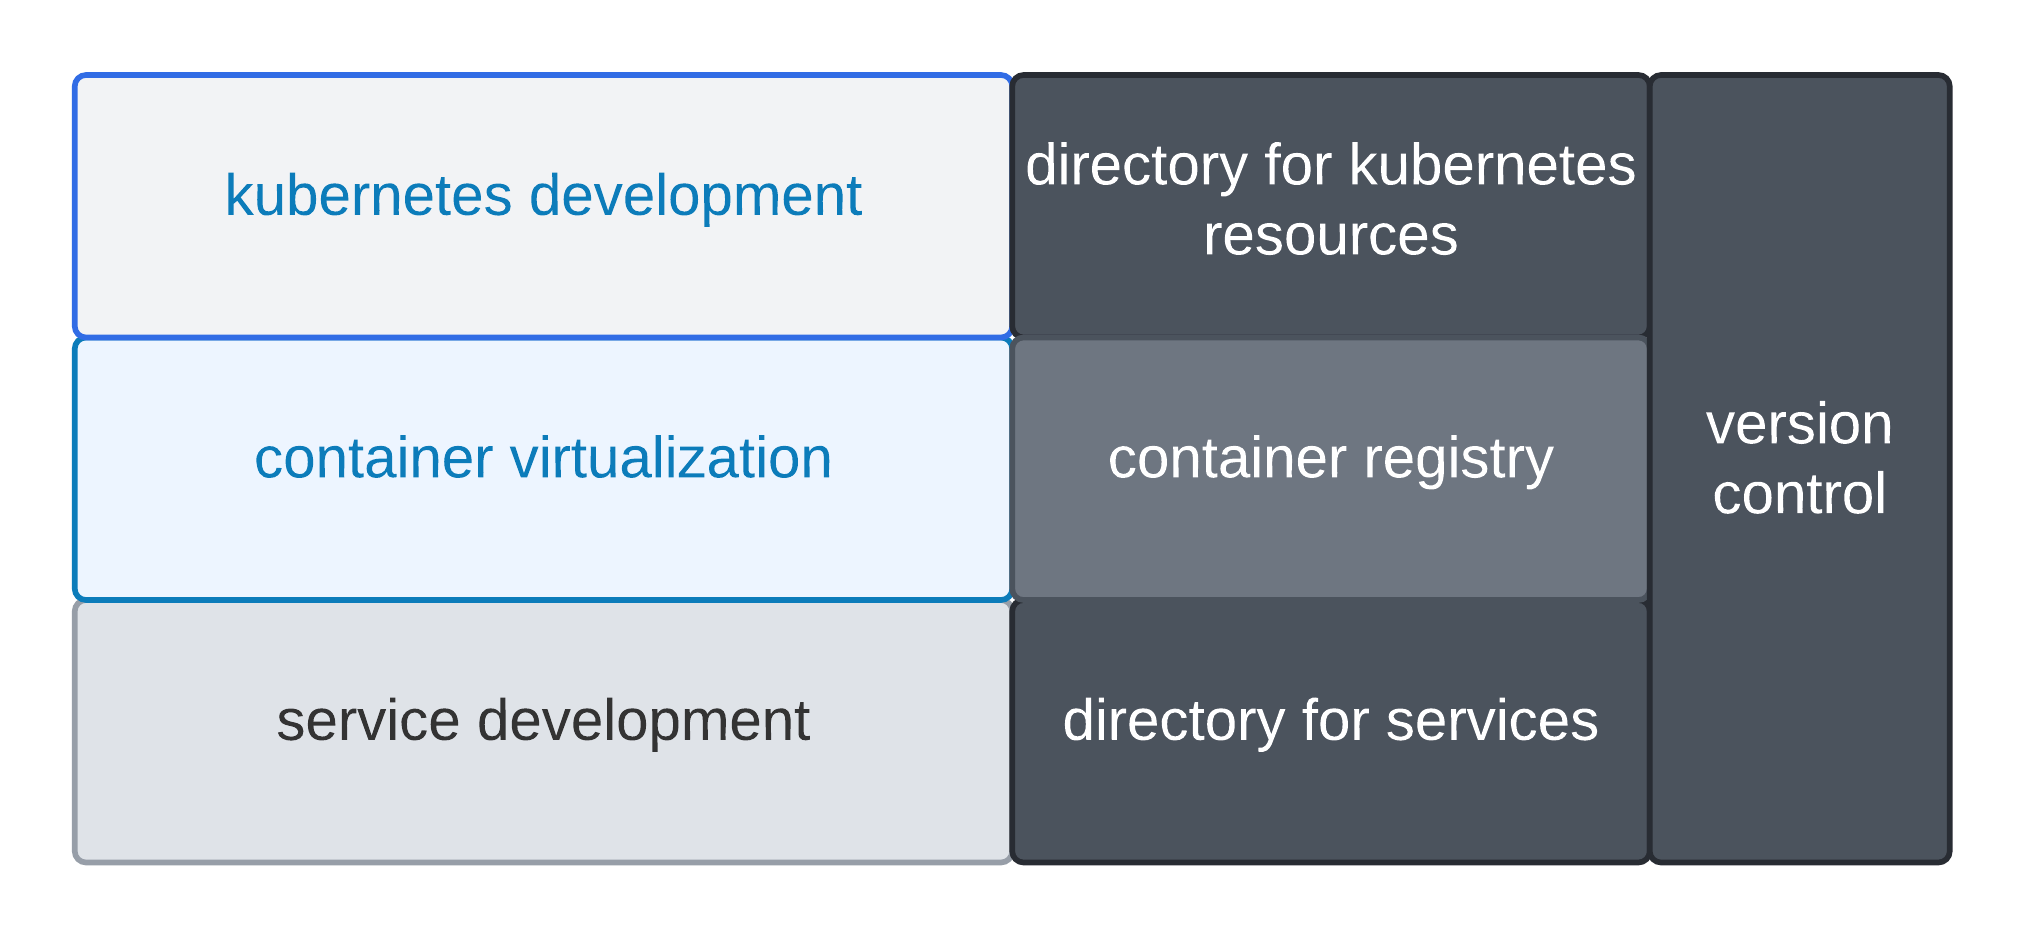
\includegraphics[width=1.0\columnwidth]{images/Schichtenentwurf.png}
    \caption{Vorgehen des Entwicklungsprozesses in Schichten}
    \label{fig:Schichtenentwurf}
  \end{figure}

\textbf{Anwendungsentwicklung}: 
Ein zentrales Repository beeinhaltet Verzeichnisse für die einzelnen Dienste.
Diese werden lokal entwickelt, getestet und ausgeführt.

\textbf{Containervirtualisierung}: 
Das entwickelte Programm wird dann containerisiert und weiterhin lokal ausgeführt.
Es wird getestet, ob die Containerisierung erfolgreich war und eine Kommmunikation untereinander möglich ist. 
Schließlich wird das Image auf ein öffentliches Registry hochgeladen. 
Jeder Dienst hat dabei einen eigenen Speicherort in Form eines Images.

\textbf{Kubernetes-Deployment}: 
Das zentrale Repository beinhaltet ein weiteres Verzeichnis für die Kubernetes-Ressourcenobjekte in Form von \acs{yaml}-Dateien.
Bei Zugang der Entwicklungsumgebung zu einem Kubernetes-Cluster können diese Dateien ausgeführt werden.

\textbf{Kubernetes-Cluster}: 
Das Testcluster wird aufgesetzt, installiert und in eine Orchestrierungsinstanz integriert.
Skripte für die Vorkonfiguration und Installation des Kubernetes-Clusters, erhalten ein eigenes Verzeichnis im zentralen Repository.
Die Auslieferung der Dienste erfolgt über das Image-Registry und werden von dem Kubernetes-Cluster heruntergeladen.



